\section{Memory-augmented Online VAD}
\label{sec:theory}

\fboxsep=1mm%padding thickness
\fboxrule=1pt%border thickness

%\begin{figure}[!t]
%            \centerline{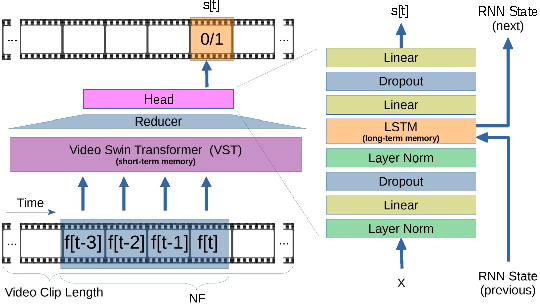
\includegraphics[clip, width=\linewidth]{images/arch-rx-cropped.pdf}}
%        \caption{The online frame-level VAD architecture. $f[t]$ is the frame at time $t$, $x$ the output of the Reducer, $\mathit{NF}$ the number of frames in input to the VST, $s[t]$ the anomaly classification score of the frame $f[t]$.\label{fig:arch}}
%\end{figure}

\begin{figure}[!t]
            \centerline{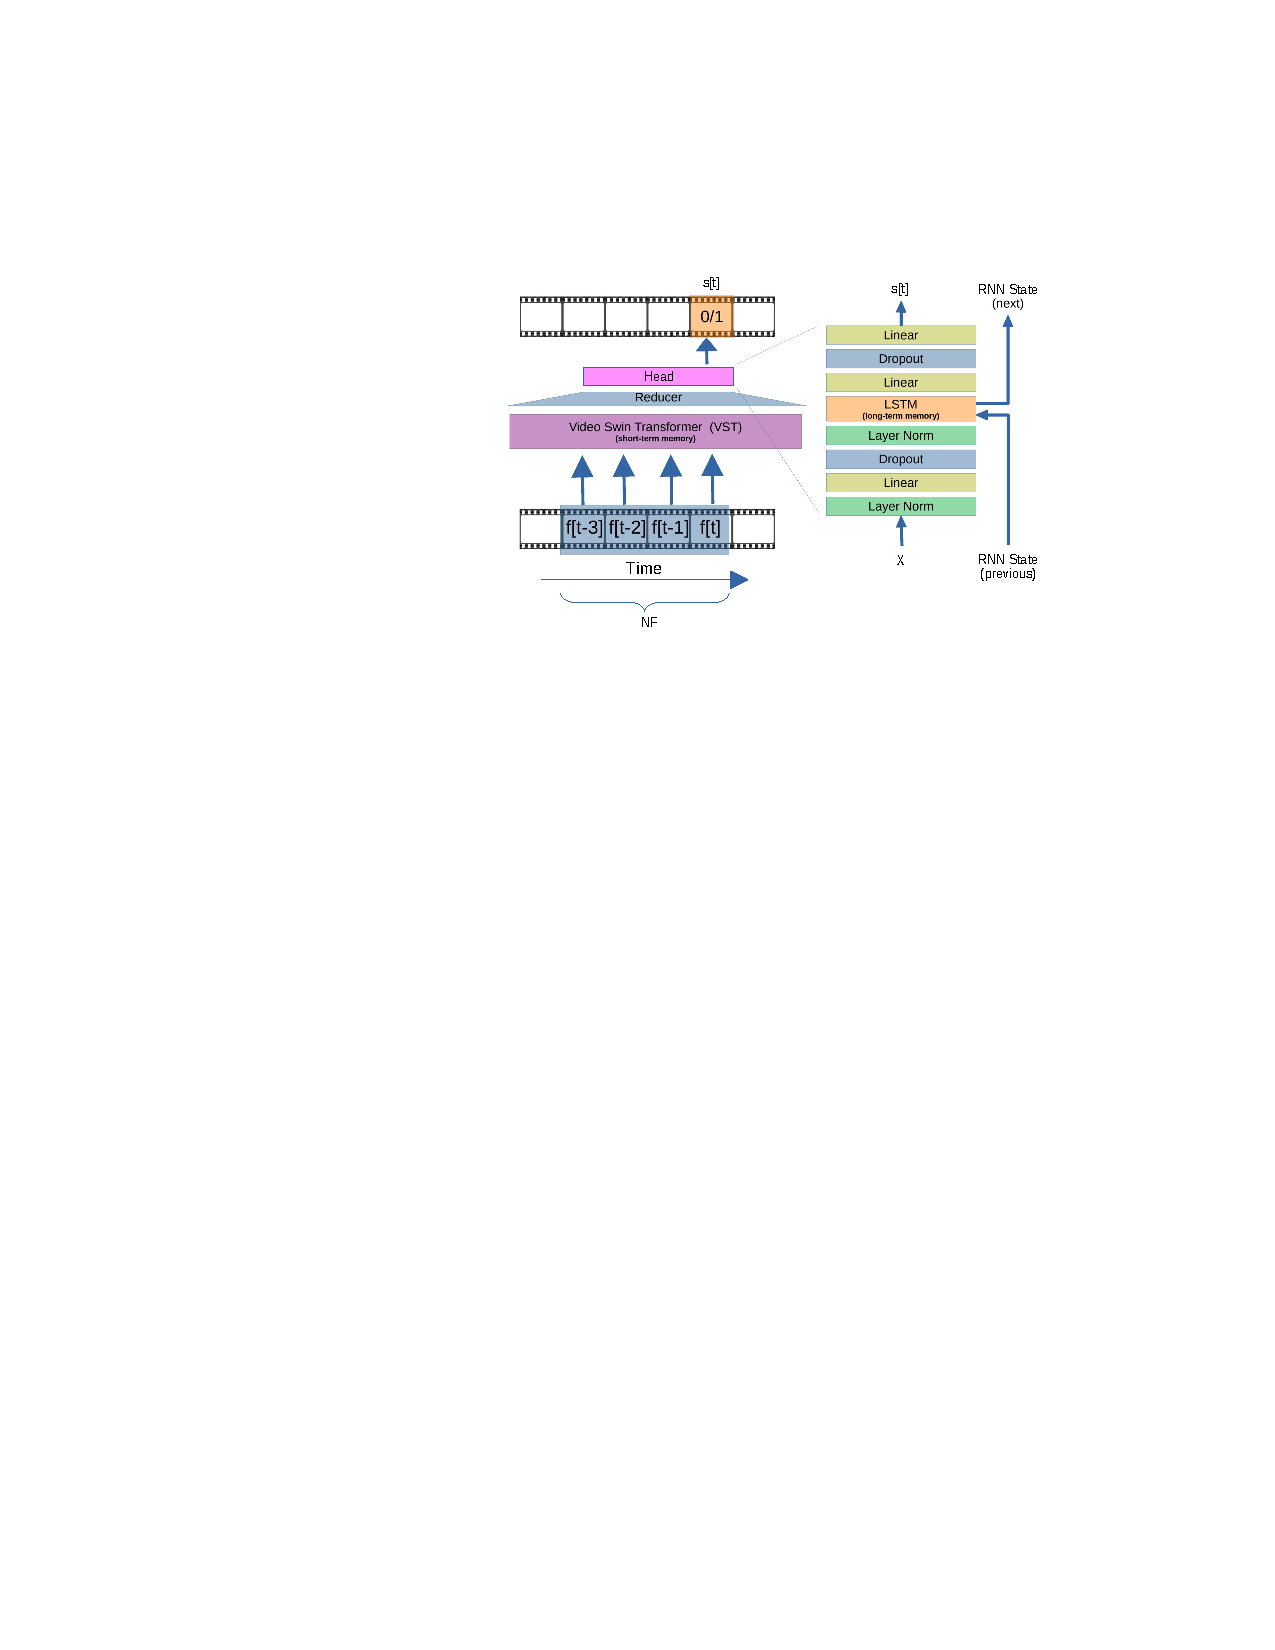
\includegraphics[clip, trim=236 510 113 133, width=\linewidth]{images/arch-rx.pdf}}
        \caption{The online frame-level VAD architecture. $f[t]$ is the frame at time $t$, $x$ the output of the Reducer, $\mathit{NF}$ the number of frames in input to the VST, $s[t]$ the anomaly classification score of frame $f[t]$.\label{fig:arch}}
\end{figure}

In our system, recently observed frames and past frames are taken into account as a source of information related to the ongoing action and the context, respectively.
In order to process current and past frames for the Online VAD task, we equipped MOVAD of two main components: a Short-Term Memory Module (STMM) and a Long-Term Memory Module (LTMM) inside the classification head (see Fig.~\ref{fig:arch}). 

\noindent\textbf{Short-Term Memory Module.}
In order to pre-elaborate the new coming frame $f[t]$ and, in conjunction, to retain near-past spatio-temporal information $f[t-1] .. f[t-\left(\mathit{NF}-1\right)]$, we chosen a transformer architecture over an RNN, to be able to process them in a parallel fashion.
We lean towards transformer over 3D convolutional models because of the well demonstrated abilities to intercept long-distance interactions in space and time \cite{moutik2023convolutional}.
We selected VST~\cite{liu_video_2022} as our backbone network for the STMM over models like ViViT~\cite{Arnab_2021_ICCV}, due to its superior performance and more efficient computation of self-attention mechanism.
%Originally VST was born to carry out the Video Action Classification task, analyzing all the frames in one step, we adapted it to perform single-frame classification using few of them. \vnote{forse si può togliere l'ultima frase}
Despite this, the self-attention mechanism remains computationally intensive, particularly for long videos. 
Therefore, we limited the input to a small temporal window of $\mathit{NF} = 4$ frames of the video, going from the current frame at time $t$ to the previous frame at time $t-\left(\mathit{NF}-1\right)$.
%small video sequences made by only 4 frames.
In this way, we obtain a compact representation of the short history that will be subsequently forwarded to the LTMM.
%In particular, a small temporal window of $\mathit{NF}$ frames of the video is considered, going from the current frame at time $t$ to the previous frame at time $t-\left(\mathit{NF}-1\right)$.
VST takes as input a video with size $\mathit{NF} \times H \times W \times 3$, where $\mathit{NF}$, $H$, $W$ and $3$ correspond to the number of frames, height, width and RGB channels, respectively.
The model internally splits the frames in non-overlapping 3D patches, partitioning the video in $\frac{\mathit{NF}}{2} \times \frac{H}{4} \times \frac{W}{4}$ 3D tokens, and using a 3D shifted window mechanism to obtain cross-window connections and exploit spatio-temporal information.

\noindent\textbf{Long-Term Memory Module.}
\label{Long-Term Memory Module descr}
As will be highlighted in ablation in Section~\ref{Short-Term Memory Module exp}, too much information about the past ($\mathit{NF} > 4$) tends to mislead the STMM, resulting in a loss of performance.
According to our hypothesis, this occurs because all frames are placed at the same level, without a possibility of weighing them based on how much they belong to the past.
For this reason, we engineered a different way to integrate and enrich the output latent space from the STMM with contextual information extrapolated from the distant past.
Every time a new frame is available, we transfer the compact representation obtained from the STMM to our LTMM, in order to update its representation of the past.
In this way, we can maintain the focus on what is happening now, and at same time accumulating a richer understanding of the scene, enabling more precise classifications.
In details, the output of VST goes through Adaptive Average Pool 3D layer (Reducer in Fig.~\ref{fig:arch}) and, finally, enters inside the classification head.
As shown in Fig.~\ref{fig:arch}, the head is composed by a series of normalization layers, linear layers and dropout, alternating. 
A stacked three-cell LSTM module is inserted after the last normalization layer to model the long-term memory.
The state, composed by three hidden $h[t]$ and cell $c[t]$ states, is updated whenever a new frame is available.
The LSTM receives in input a features block of $[B, 1024]$, where $B$ is the batch size, and returns a block of same size together with the state of the cells.
Since the state is relatively small, the module is very efficient and leads to a fixed and limited additional computational cost.
For each frame $f[t]$, the classification head outputs the anomaly classification score $s[t] \in [0,1]$, where $0$ means no anomaly and $1$ means the frame is anomalous.
A weighted cross-entropy loss was chosen to train the model, giving higher weight to the anomaly class reflecting the distribution of the data.
For each weight $w_i$, we used the formula $w_i = e / e_i$, where $e$ the total amount of examples in the dataset and $e_i$ the amount of examples for the class $i$.

% copyright image frame: <a href="https://www.freepik.com/free-vector/realistic-vector-icon-film-tape-strip-with-white-square-isolated-white-cinema-concept_31096470.htm#query=video%20frame&position=31&from_view=keyword">Image by user15245033</a> on Freepik